Las imágenes en tonos de grises (por ejemplo, una foto en blanco y negro)
son matrices de valores entre 0 y 255.
Cada elemento de la matriz se denomina \emph{píxel}.
El valor 0 representa el negro, el 255 el blanco, y los valores intermedios
las distintas intensidades de grises.

\begin{center}
  \begin{tikzpicture}[yscale=-1, scale=.10]
    \begin{scope}
      \node[anchor=north west, inner sep=0pt] at (0, 0) {
\includegraphics[scale=5.9]{arreglo-imagen/utfsm.png}};
      \draw[very thin] (0, 0) grid (45, 27);
      \draw[step=3cm] (0, 0) grid (45, 27);
      \node[ultra thick, draw=red!80!black, inner sep=5pt] (A) at (34.5, 19.5) {};
      \node[anchor=north] at ({45 / 2}, 27) {\texttt{img}};
    \end{scope}
    \begin{scope}[xshift=65cm, yshift=18cm]
      \node[anchor=north west, inner sep=0pt] at (0, 0) {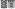
\includegraphics[scale=5.87]{arreglo-imagen/utfsm-chica.png}};
      \draw[very thin] (0, 0) grid (15, 9);
      \node[very thick, draw=red!80!black, inner sep=2pt] (B) at (11.5, 6.5) {};
      \node[anchor=north] at ({15 / 2}, 9) {\texttt{reducir(img, 3)}};
    \end{scope}
    \begin{scope}[xshift=100cm]
      \node[anchor=north west, inner sep=0pt] at (0, 0) {
\includegraphics[scale=5.89]{arreglo-imagen/utfsm-bin.png}};
      \draw[very thin] (0, 0) grid (45, 27);
      \node[anchor=north] at ({45 / 2}, 27) {\texttt{binarizar(img, 146)}};
    \end{scope}
    \draw[very thick, -latex'] (A) to (B);
    %\draw[very thick, -latex', out=180] (A.north east) to (B.north west);
    %\draw[very thick, out=-45, in=-145, -latex'] (A.north east) to (B.north west);
  \end{tikzpicture}
\end{center}

\begin{enumerate}
  \item
    Un método para reducir \(f\) veces el tamaño de una imagen
    es partir la imagen en bloques de \(f\times f\)
    y promediar los valores de los píxeles de cada bloque.
    Este promedio será el valor del píxel correspondiente en la nueva imagen.
    Si la imagen original es de \(m\times n\) píxeles,
    la imagen reducida quedará de \((m/f) \times (n/f)\) píxeles.

    Escriba la función \li!reducir(img, f)!,
    donde \li!img! es una imagen (es decir, una matriz),
    que retorne una nueva imagen
    que sea \li!img! reducida en un factor de \li!f!.

  \item
    La \emph{binarización} de una imagen
    consiste en crear una nueva imagen cuyos píxeles sólo son negros o blancos.
    Para esto se escoge un valor llamado \emph{umbral};
    todos los píxeles mayores o iguales que el umbral quedan blancos,
    y los menores al umbral quedan negros.

    Escriba la función \li!binarizar(img, umbral)!
    que retorne una nueva imagen
    que sea una versión binarizada de \li!img! de acuerdo al umbral indicado.
\end{enumerate}

